\section{Rollback and compensation are different operations}\label{sec:C32:04}
Rollback restores a prior software or logical state. Compensation attempts to counteract an external effect using another operation. Neither necessarily reconstructs the world that existed before the original action. Deleting a published object may not undo its disclosure; reversing a financial transaction may not remove fees or downstream actions; restoring a database snapshot can erase legitimate concurrent writes. An agent runtime must classify which effects are reversible, compensatable, or irreversible under the actual service contract.

Consider a hypothetical enterprise agent that prepares a report, uploads it, then records the uploaded identifier in memory. The service accepts an idempotency key. The following failure sequence is possible:
\begin{table}[!htbp]
\centering
\caption{Constructed upload failure and effect-reconciliation sequence.}\label{tab:C32:recovery}
\begin{tabular}{L{0.12\linewidth}L{0.38\linewidth}L{0.35\linewidth}}

\toprule Step & Durable evidence & Recovery implication\\\midrule
1 & Intent and operation key stored & The intended effect is identifiable after restart.\\
2 & Upload request submitted & Submission alone does not prove the final state.\\
3 & Service commits; response lost & Local timeout leaves outcome unknown.\\
4 & Process crashes before memory write & Session history omits the completed effect.\\
5 & Runtime resumes & Query by operation key before deciding whether to retry.\\
6 & Committed object found & Record reconciled outcome; do not create a duplicate.\\
\bottomrule
\end{tabular}
\end{table}
The correct recovery cannot be inferred from a natural-language summary that says upload failed. It requires operation identity and reconciliation semantics. If the service lacks idempotency and lookup, a global exactly-once claim is unsupported. The application may need conservative escalation, an outbox pattern with a specialized delivery service, or a bounded duplicate-risk policy. These are explicit changes to the operating contract.

Idempotency is a scoped service property. The same logical operation must retain its identity across retries, and reuse of an identifier with different arguments must follow a declared conflict rule. Deduplication retention, namespace, concurrent submission and crash behavior determine how long the protection holds. Expiry of a deduplication record can make an old delayed retry appear new. HTTP's idempotent-method semantics concern the intended effect of repeated identical requests, not a universal exactly-once execution or identical-response promise~\cite{cumulative_c_http9110}. A client therefore needs the actual application's operation contract before retrying a non-idempotent effect. A local outbox can durably retain intent while delivery remains repeated; the receiving service still determines whether those deliveries become duplicate effects.

Memory rollback must preserve authority monotonicity. Suppose a credential was revoked after a checkpoint. Restoring that checkpoint must not restore the old credential's authority. Revocation information should be applied from an authoritative current source even when task state is rolled back. The same principle applies to deletion tombstones and legal retention boundaries: an old backup is not permission to resurrect information for use. Recovery is a compatibility-preserving reconstruction under current authority, not unconditional time travel.

The three contracts in Chapter~\ref{ch:C01} apply at different points in this reconstruction. A byte-faithful checkpoint may preserve old proposal conditioning while violating current authority. A permission-filtered restoration may preserve authority while changing proposal probabilities. Reconciliation may legitimately update an unknown effect status after obtaining new service evidence; that update must be distinguished from the preceding representation-only restoration. The recovery trace should therefore record restoration, current-authority filtering, and external reconciliation as separate typed transitions. Testing only equality with the old snapshot would reward the wrong behavior after revocation.

For a rollback from $\nu_1$ to $\nu_0$, the required condition is not simply that old code starts. There must be an admissible conversion $\psi$ such that
\begin{equation}
 \mathsf C(\nu_0,\psi(S_1))=1,
\end{equation}
while external effects and current authorization remain reconciled. A lossy forward migration may have no inverse. The release procedure must then retain a recoverable representation or declare the rollback boundary before deployment. Pretending every schema migration is reversible converts a known design limitation into an incident.



Figure~\ref{fig:C32:overview} isolates the mechanism and its stated information boundaries.
\begin{figure}[!htbp]
\centering
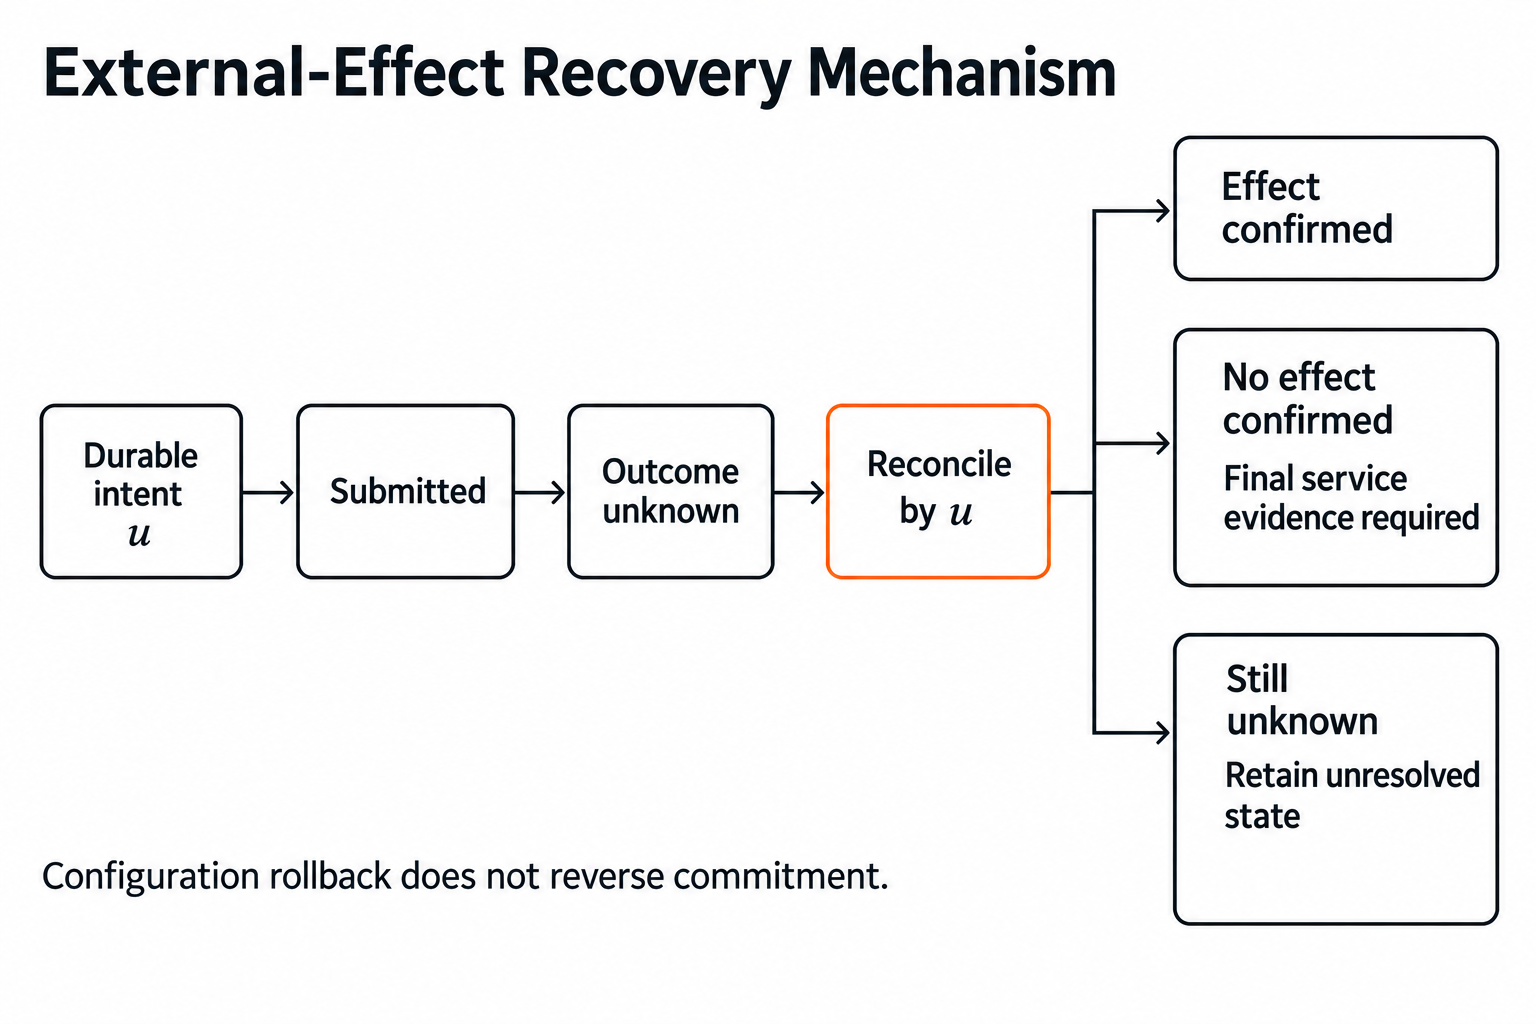
\includegraphics[width=\linewidth]{book/figures/assets/F32review.png}
\caption{Recovery retains operation identity and distinguishes submission from commitment evidence. A missing receipt does not prove absence. Only the service contract can justify a confirmed effect or a final negative outcome; otherwise the ledger stays unresolved. Configuration rollback does not reverse an external effect.}
\label{fig:C32:overview}
\end{figure}
